\label{sec:dataset}
\section{Data set exploration}

The job offers corpus contains 8565 job offers written in French, English, German, and Italian and contains positions from a wide range of Swiss cantons. Below is a description of each variable in the job offers data set:

\textbf{JOB ID}: A unique numerical identifier assigned to each job offer in the corpus.

\textbf{ISCO}: An identifier that relates the job posting to the Swiss Standard 	
Classification of Occupations (CH-ISCO-19). This fact sheet is published by the Federal
Statistical Office and is used for several federal labour market surveys. 

\textbf{SKILLS}: A list of text keywords describing the skills, sectors, or industries related to each job offer.

\textbf{CANTON}:The canton the job offer was originally advertised in. 

\textbf{WORK EXPERIENCE}: A list of keywords describing job titles related to each job offer.

\textbf{EDUCATIONAL LEVEL}: The educational experience desired by each job offer.

\textbf{DATE}: The date the job offer was published. 

\textbf{COMPANY}: The name of the company advertising the job offer. 

\textbf{JOB TITLE}: The official job title of the job offer. 

\textbf{JOBS}: A list of keywords related to the official job title.

\textbf{CONTENT}: The raw text of the job offer, written in French, English, German, Italian, or some combination. 

Data sets of environmentally-related skills and activities were also compiled by the GE-EN-VIE researchers in order to create reference documents to match the contents of the job offers to. Below of is a description of the activities data set:

\textbf{ACTIVITY ID}: A unique numerical ID assigned to each environmentally related activity.

\textbf{O*Net - All the jobs}: A short list of broad keywords that describe the category of skills the detailed activities fall under. 

\textbf{O*Net - Green jobs}: A unique numerical ID assigned to each activity description.

\textbf{O*Net - Details of the activities for green jobs }: A sentence describing each occupational activity in detail, as listed in the O*Net database. 

\textbf{Terms (verbs) found in the 120 "environment" job offers}: A list of individual verbs related to the sentences of detailed activities.

\textbf{Terms (adjectives) found in the 120 "environment" job offers}: A list of individual adjectives related to the sentences of detailed activities. 

The description of the data set of the environmentally-related skills is as follows: 

\textbf{SKILL ID}: A unique numerical ID assigned to each environmentally related skill.

\textbf{SKILL}:  A sentence describing each occupational skill in detail, as listed in the O*Net database. 

To assist with the automatic classification of environmentally related and non-environmentally related jobs, a total of 536 jobs were manually labeled as such by Marie-José Genolet Viaccoz. In addition, a total of 1000 jobs from the job offers corpus were analyzed in an exploratory analysis to gain a better understanding of the data set. 

The distribution of jobs by location, shown per canton in Switzerland, is shown in Fig.~\ref{fig:cantons}. The majority of the jobs postings are for positions in Bern and Vaud, followed by Geneva. Of all the cantons, Geneva has the highest ratio of environmental jobs to non-environmental jobs. 

\begin{figure}[htbp]
  \centering
    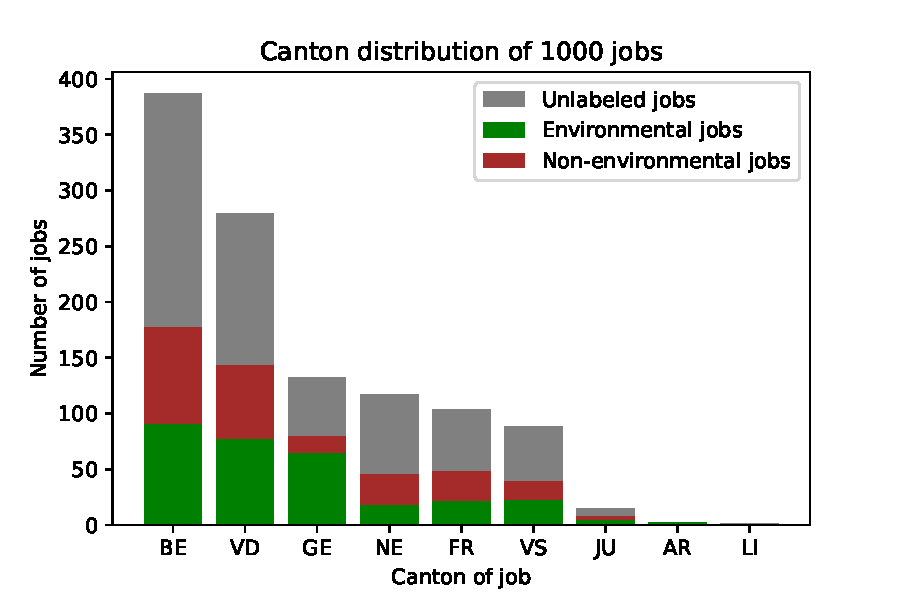
\includegraphics[width=0.49\textwidth]{figures/CantonDist.pdf}
    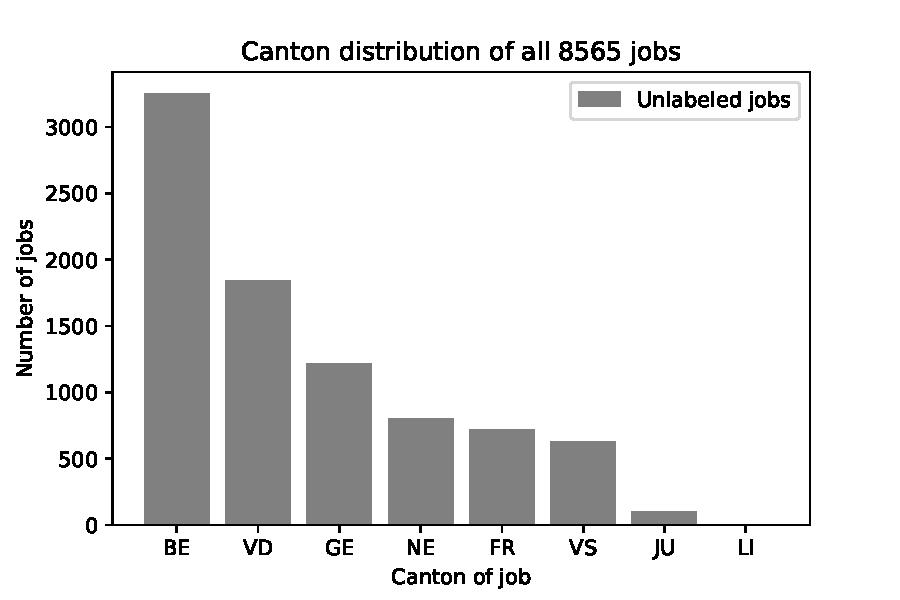
\includegraphics[width=0.49\textwidth]{figures/CantonDistAll.pdf}
    \caption[The distribution of job locations by canton in Switzerland]{
    	The distribution of job locations by canton in Switzerland.
        The left plot shows a subset of 1000 jobs, of which nearly half are labeled to indicate if they are environmental. The right plot shows the distribution for all 8565 jobs.
        Jobs categorized as environmental are shown in green, and those that are not environmental are shown in red.
        The portion of the data set that has not been categorized is shown in grey. The right plot shows the distribution
        of all 8565 jobs in the data set.
    }
\label{fig:cantons}
\end{figure}

Most of the jobs in the data set were sourced from small or midsize companies. The proportion of environmentally related jobs to non-environmentally related jobs is relatively consistent across company size, as seen in Fig.~\ref{fig:companysize}.

\begin{figure}[htbp]
  \centering
    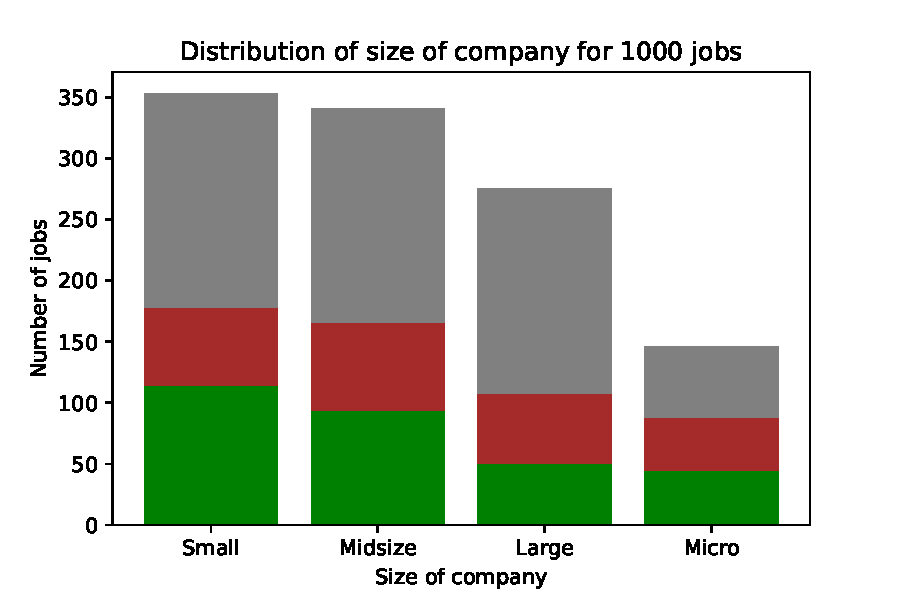
\includegraphics[width=0.49\textwidth]{figures/CompanySize.pdf}
    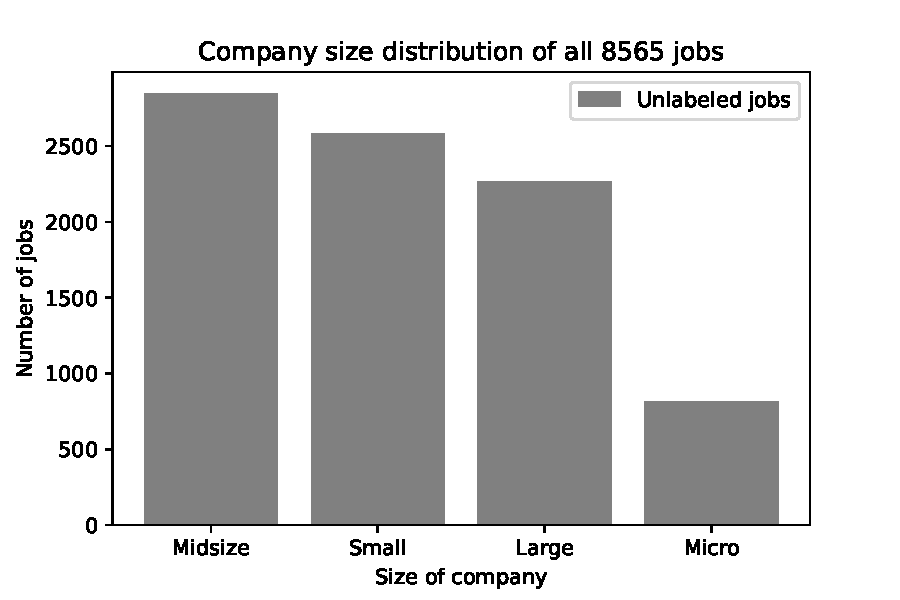
\includegraphics[width=0.49\textwidth]{figures/CompanySizeAll.pdf}

    \caption[The distribution of company size in the jobs data set]{
    	The distribution of company size.
    	The left plot shows a subset of 1000 jobs, of which nearly half are labeled to indicate if they are environmental. The right plot shows the distribution for all 8565 jobs.
        Jobs categorized as environmental are shown in green, and those that are not environmental are shown in red.
        The portion of the data set that has not been categorized is shown in grey. The right plot shows the distribution
        of all 8565 jobs in the data set.
    }
\label{fig:companysize}
\end{figure}



With regards to the number of sentences in each job description, a greater number of non-environmentally related jobs had descriptions with fewer sentences, as seen in Fig.~\ref{fig:sentencelength}. Many of these job descriptions do not contain enough information about the job or company to be classified as environmentally related.


\begin{figure}[htbp]
  \centering
    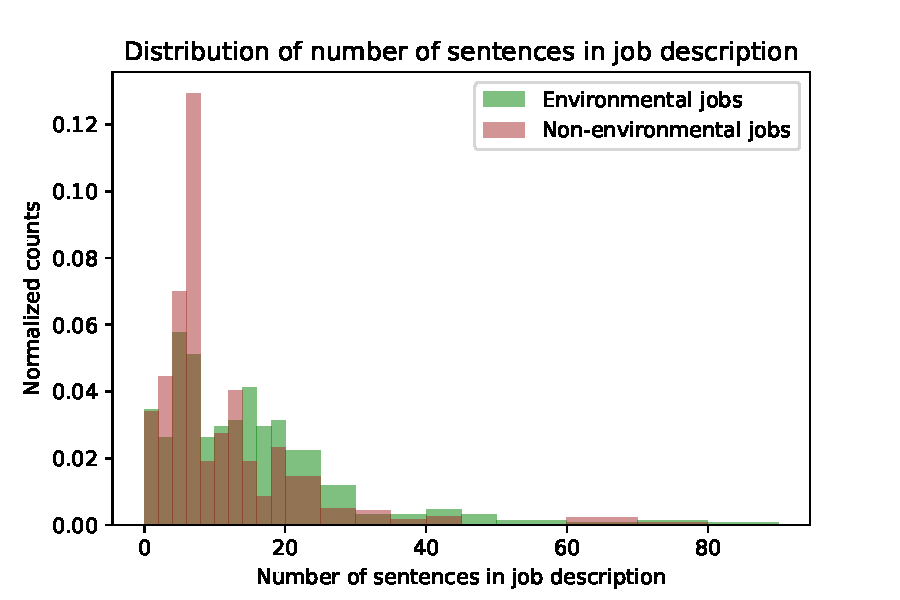
\includegraphics[width=0.49\textwidth]{figures/SentenceLength.pdf}
    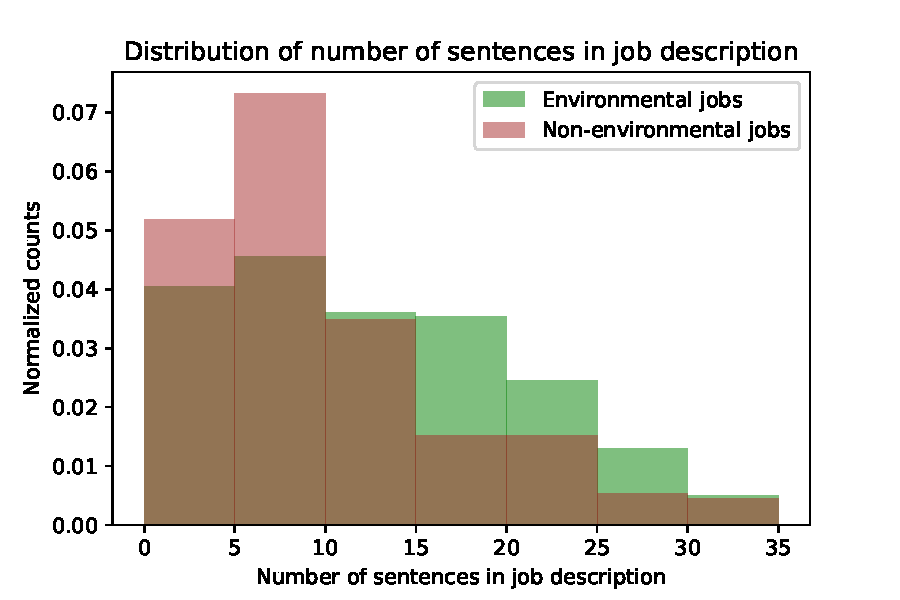
\includegraphics[width=0.49\textwidth]{figures/SentenceLengthZoomed.pdf}

    \caption[The distribution of the number of sentences in each job description]{
    	The distribution of the number of sentences in each job description.
    	The left plot shows the densities of the 536 labeled jobs. The right plot shows the same subset of jobs, but on a range from 0-35 sentences. 
        Jobs categorized as environmental are shown in green, and those that are not environmental are shown in red.
    }
\label{fig:sentencelength}
\end{figure}


The distribution of the number of sentences in the entire data set is similar to that of the subset of 536 labeled job offers, as seen in Fig.~\ref{fig:sentencelengthall}. The vast majority of the job offers contain fewer than 20 sentences. 

\begin{figure}[htbp]
  \centering
    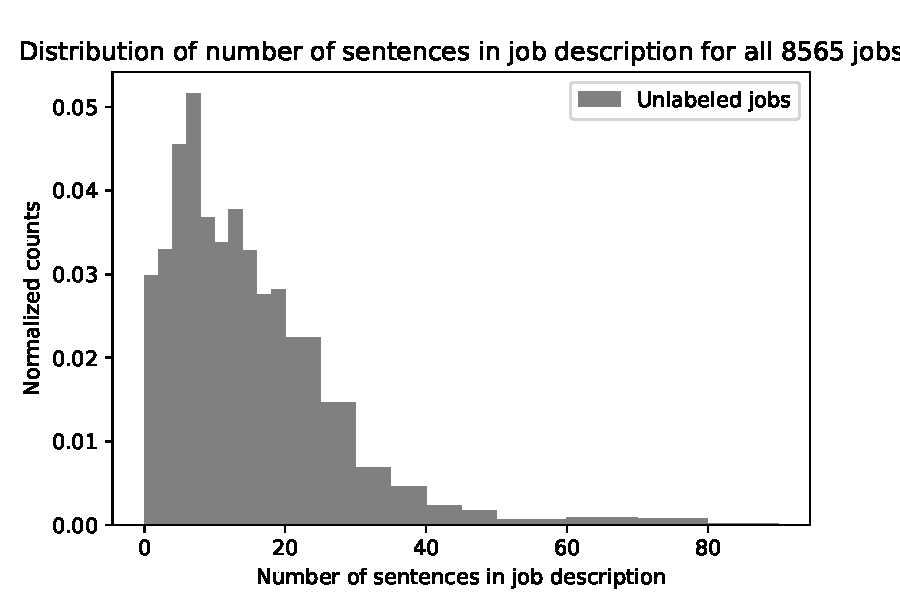
\includegraphics[width=0.49\textwidth]{figures/SentenceLengthAll.pdf}
    \caption{
    	The distribution of the number of sentences in all 8565 job descriptions.
    }
\label{fig:sentencelengthall}
\end{figure}


A large number of job descriptions in the data set have fewer than 200 characters as seen in Fig.~\ref{fig:charlength}. Likewise, as with the number of sentences, job descriptions with small amounts of text are more frequently classified as as non-environmentally related.

\begin{figure}[htbp]
  \centering
    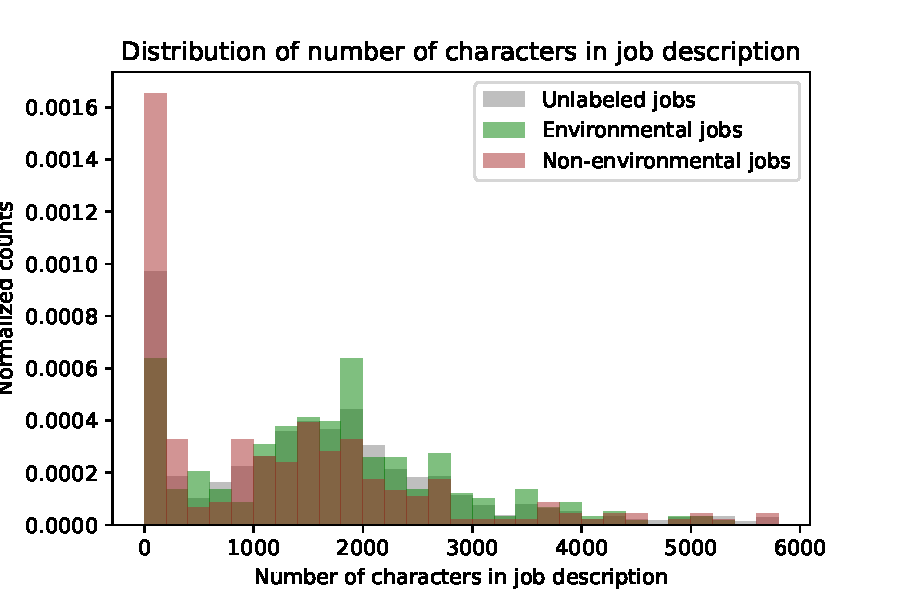
\includegraphics[width=0.49\textwidth]{figures/CharLengthZoomed.pdf}
    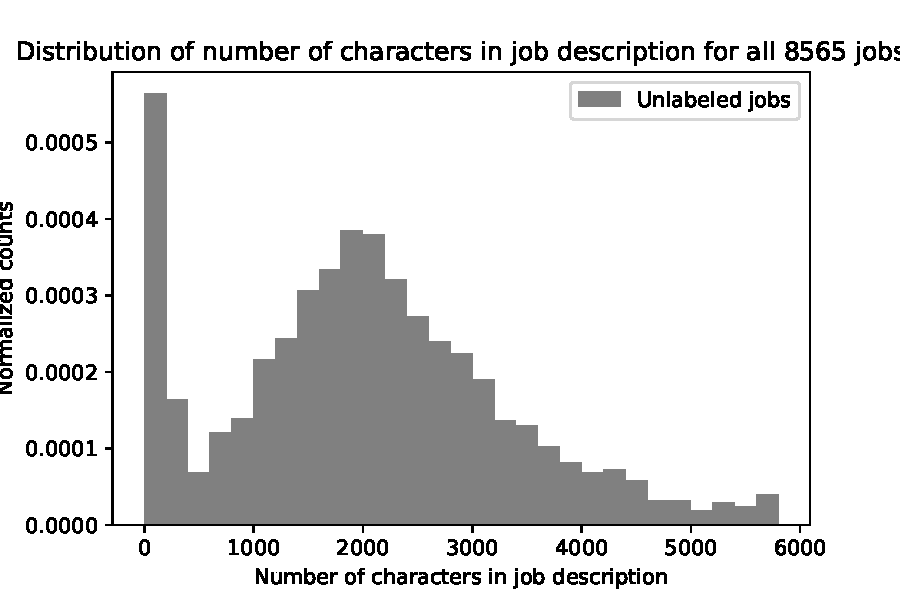
\includegraphics[width=0.49\textwidth]{figures/CharLengthAll.pdf}

    \caption[The distribution of the number of characters in each job description]{
    	The distribution of the number of characters in each job description.
    	The left plot shows the character densities of the 536 labeled jobs. The right plot shows the character densities for all 8568 jobs. 
        Jobs categorized as environmental are shown in green, and those that are not environmental are shown in red. Unlabeled jobs are in grey. 
    }
\label{fig:charlength}
\end{figure}
